
\section*{Part 3}

\subsection*{a) i}
\textbf{Implement a solver of equation (3) on the preceding page for N atoms, given initial positions
and velocities.
}
This was taken care of from the start, no changes needed.

\subsection*{a) ii}
\textbf{Use Newton’s third law to reduce the number of force calculations.
}
Newtons third law states that if a particle A exerts a force on another particle B, there must be an equal force acting in the other direction. We can take advantage of this by completing $A \rightarrow B$ when we have calculated $B \rightarrow A$.

In practise this means taking the cartesian product of all the particles , ignoring the diagonal (because A does not exert a force on itself.) In practise we only need to consider what is above and to the right of the diagonal.

In the code this has been implemented in the VelocityVerletFast algorithm. 


\subsection*{a) iii}
\textbf{Extend your implementation such that atoms more than $3\sigma$ apart do not interact}
The velocityVerletFast implementation also ignores particles that are more than $3 \sigma$ distance. It takes advantage of the fact that a cartesian matrix is mirrored around the diagonal. Therefore we can both ignore the diagonal (particles do not self-interact) and use only the upper triangle.


\subsection*{iv}
\textbf{Plot the shifted potential and the corresponding force to verify your implementation of the
cut-off.}

The shifted potential ensures that the force is a little weaker than the Lennard Jones potential. Because the LJ potential is itself an approximation, its ok to tinker with it a little bit. The benefit of a shifted potential is that there is a continous progression close to $3 \sigma $ and beyond it.

\begin{figure}[h!]
        \centering 
        %Scale angir størrelsen på bildet. Bildefilen må ligge i samme mappe som tex-filen. 
        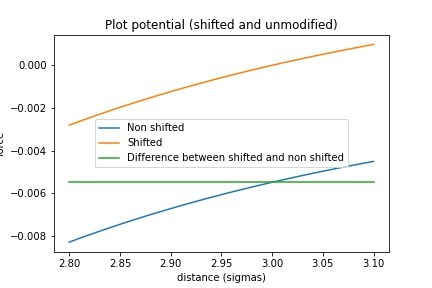
\includegraphics[scale=0.6]{./py/plotPotentialDiff.jpg} 
        \caption{Shifted  Lennard Jones  potential becomes 0 at exactly $3\sigma$, allows cutoff at this range }
        %Label gjør det enkelt å referere til ulike bilder.
        \label{fig:eksempelbilde1}
\end{figure}

\subsection*{a) v}
\textbf{Does the shift of the potential described above impact the force calculations?}
Because the potential is a constant, it does not affect the derivative, i.e the slope of the curve. The force is simply set to zero a little earlier. This makes any effects of the attractive force at distances greater than the cutoff length nil. This could obviously be bad, but in most cases there is a range in which this doesn't matter, either because it's too weak, or because it is crowded out by many more and stronger attractions from closer particles. The shift also makes the repulsive force kick in a little bit sooner. This part of the potential is so steep anyway that it doesn't make a difference in practise. 

Note that the shifted potential doesn't affect how the particles are accelerated, when in range. It only shifts the position slightly when they are affected.


\subsection*{3b) i}
\textbf{Reproduce your results for the 2-atom model from the previous section to verify your implementation.}

Comparing the xyz files produces by the optimized VelocityVerlet and the non-optimised gives results that are indistinguishable upon inspection.

\subsection*{3b) ii}
\textbf{Simulate the motion of four atoms starting at rest from the positions}
This was been done.

\subsection*{3b) iii}
\textbf{Visualise the results in Ovito, describe and explain the motion.}

The atoms remain in a steady state, perfectly positioned in a square. They move inwards and outwards slowly, and but being pulled toward the through in the potential. The reason is that the starting distance is very close to the distance of the the through.


\begin{figure}[h!]
        \centering 
        %Scale angir størrelsen på bildet. Bildefilen må ligge i samme mappe som tex-filen. 
        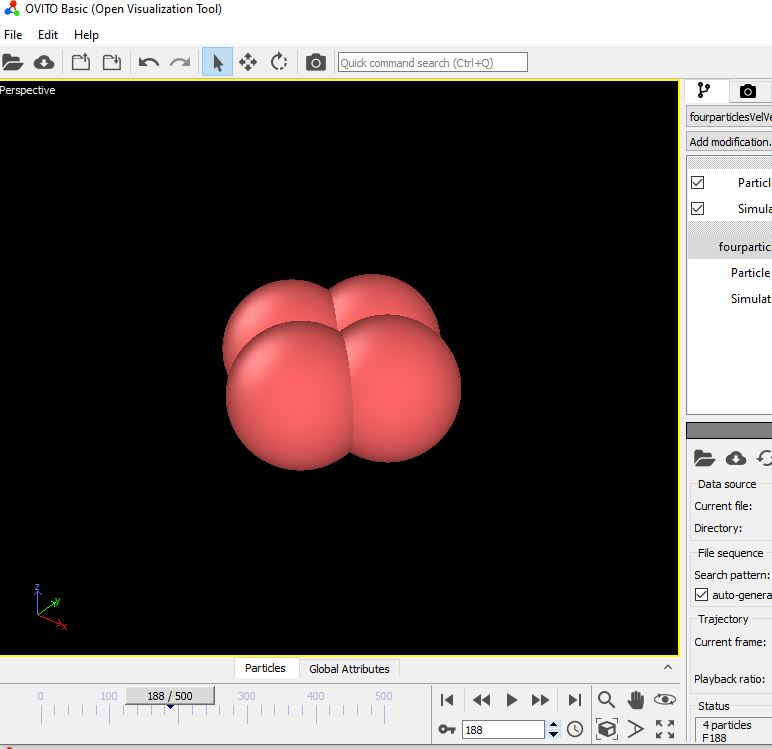
\includegraphics[scale=0.6]{./py/3biii_ovito.jpg} 
        \caption{Four particles visualised in Ovito}
        %Label gjør det enkelt å referere til ulike bilder.
        \label{fig:3biii}
\end{figure}


\subsection*{3b)iv}
\textbf{Plot the potential, kinetic and total energy as a function of time, and comment on the energy
conservation}

We plot the energies, and see that there are no runaway accumulation or leak. The energy is conserved.

\begin{figure}[h!]
        \centering 
        %Scale angir størrelsen på bildet. Bildefilen må ligge i samme mappe som tex-filen. 
        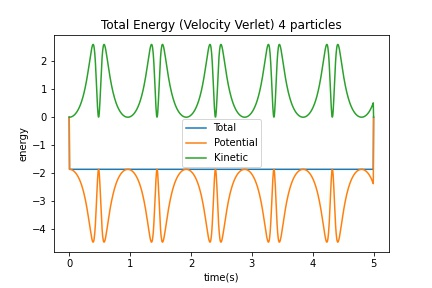
\includegraphics[scale=0.6]{./py/3b_iv.jpg} 
        \caption{256 atoms energy}
        %Label gjør det enkelt å referere til ulike bilder.
        \label{fig:3biv}
\end{figure}

\subsection*{3b)v}
\textbf{Repeat the above exercises with a small perturbation in the initial positions, such that the first
atom starts at}
We repeat it with a small perturbation, ans immediately see a large amount of randomness emerge. The introduction of the perturbation makes the movement chaotic, and it becomes much harder to tell if there is a leak. It's therefore a good idea to check the integrity of energy conservation using simpler setups.


\begin{figure}[h!]
        \centering 
        %Scale angir størrelsen på bildet. Bildefilen må ligge i samme mappe som tex-filen. 
        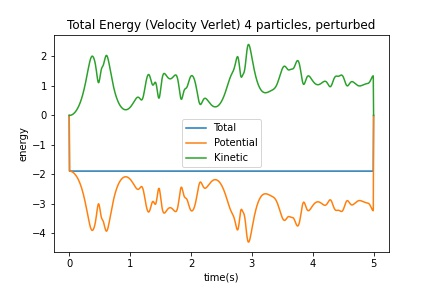
\includegraphics[scale=0.6]{./py/3b_v.jpg} 
        \caption{Total energy between four atoms }
        %Label gjør det enkelt å referere til ulike bilder.
        \label{fig:3biv}
\end{figure}

\subsection*{3c) i}
\textbf{Write a function which takes n and L (or n and d) as arguments and returns the positions of 4n
3
atoms on a face-centred cubic lattice.
}

I have made a function in the  \textbf{MDGennerators} modules, named \textbf{PopulateCreateCrystalStructure}(3, 1). This takes as an argument the number of unit cells and the distance between them. Each cell contains four tetrahedrally placed Argon atoms.

\subsection*{3c) ii}
\textbf{Verify your implementation by calling your function for n = 3 and L = 20, writing the resulting
positions to an xyz-file and looking at the result in Ovito. Your system should contain 4 · 3
3 = 108
atoms.}

Verifying that there are 108 particles in the crytal.

\subsection*{3c) iii}
\textbf{Show that the unit cell size corresponding to the density $\rho = 1.374 g/cm3$
is $d = 1.7\sigma$ This will be used in the remaining parts of the project.}

Reasoning : The unit cell size corresponding to 1.374 g per $cm^3$ must be equal to the mass of the atom Argon, multiplied with the number of particles that fit within 1 $cm^3$.

In order for the mass to be 1.375 grams per cubic centimeter, the number of unit cells containing four atoms in one centimeter must be known, and the mass of each atom must be known. 


\begin{equation}
4m \cdot  n^3 = 1.375 g/cm^3
\end{equation}

The distance for  $\sigma $ that is associated with this density, we name $\sigma_d$, and it can be expressed as the $1 cm / n$. Hence, converting the centimeter to meters units, $\sigma_d$ must be given by :


\begin{equation}
\sigma_d= \frac{0.01}{n}
\end{equation}

We were told that the value for $\sigma$ for Argon was $3.405Å$. Hence, our value for $\sigma_d$ should be exactly $3.405 \cdot 1.7 Å$.Expected value for $\sigma_d = 3.405 \cdot 1.7 = 5.7885 Å$

We must now find the value for $n$. , 
\begin{equation}
4m \cdot  n^3 = \frac{1.375 g}{1 cm^3} 
\end{equation}


We were given the mass $m$ of Argon as $m = 39.95 u, u = 1.66 \cdot 10^{-27}g$, which is then 

\begin{equation}
39.95 \cdot 1.66 \cdot 10^{-27} = 6.6317E-26 g 
\end{equation}

This equation then gives us

\begin{equation}
4(6.6317 \cdot 10^{-26} g ) \cdot  n^3 = \frac{1.375 g}{1 cm^3}
\end{equation}

Solving this for $n$ using tools should give us the number of unit squares per cm.

\begin{equation}
n =\sqrt[3]{\frac{5^{26}\cdot \:23068672}{6.6317}} = 173063684.30366
\end{equation}

Dividing this cm into 173063684.30366 units, and converting the distance to Ångstrøm units,  gives us:

\begin{equation}
\sigma_d = \frac{1}{173063684.30366} \cdot  10^{9} = 5.778219 Å
\end{equation}


When multiplying to get the size in Ångstrøms, we multiply with $10^9$, because this is 10 magnitudes increase from 1, the initial 10. This is another 9 magnitudes. This shows that we get the same value as expected. We have thus connected the mass of the molecule, distance between unit cells $\sigma$ and the density.

We will now use the $\sigma_d = 1.7 $ for the remainder of the project.



\subsection*{3d) ii}
\textbf{Simulate 256 atoms starting from rest, and visualise the result}

I have simulated with 256 atoms, creating this crystal structure

\begin{figure}[h!]
        \centering 
        %Scale angir størrelsen på bildet. Bildefilen må ligge i samme mappe som tex-filen. 
        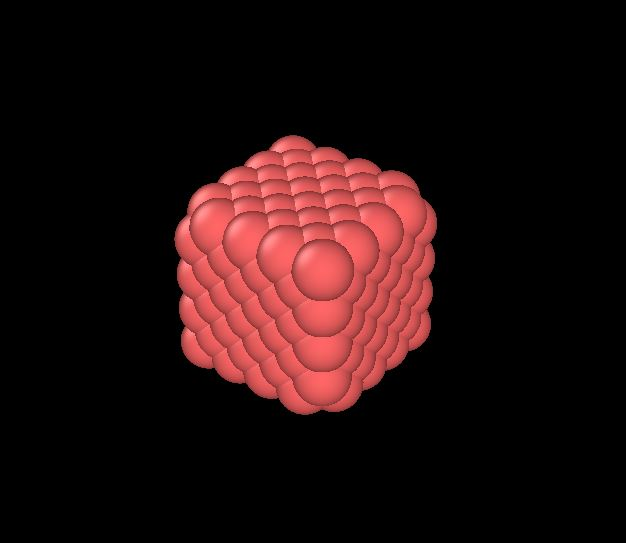
\includegraphics[scale=0.6]{./py/3di_1_ovito.jpg} 
        \caption{Crystal lattice }
        %Label gjør det enkelt å referere til ulike bilder.
        \label{fig:3di_1}
\end{figure}


\subsection*{3d) ii}
\textbf{Plot the potential, kinetic and total energy as a function of time. What is the main difference
from the energy graphs for two and four atoms?
}

The difference is apparent. The more atoms, the more forces are acting between the particles. The net result is that variations in positions are smaller. This can also be interpreted as higher number of close particles, means higher probability of interacting with those particles.

\begin{figure}[h!]
        \centering 
        %Scale angir størrelsen på bildet. Bildefilen må ligge i samme mappe som tex-filen. 
        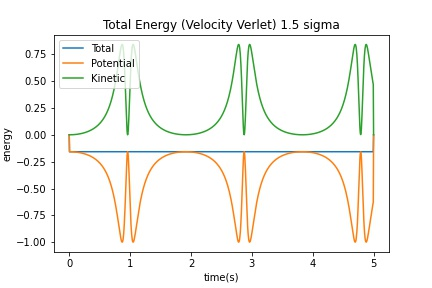
\includegraphics[scale=0.6]{./py/3dii_energy_two.jpg} 
        \caption{Energy for two atoms}
        %Label gjør det enkelt å referere til ulike bilder.
        \label{fig:3di_2}
\end{figure}
\begin{figure}[h!]
        \centering 
        %Scale angir størrelsen på bildet. Bildefilen må ligge i samme mappe som tex-filen. 
        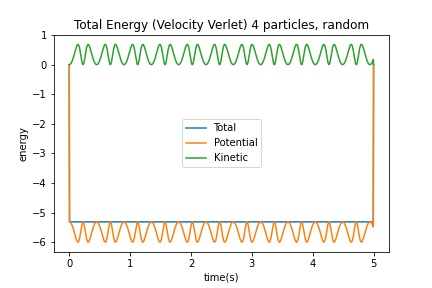
\includegraphics[scale=0.6]{./py/3dii_energy_four.jpg} 
        \caption{Energy for four atoms}
        %Label gjør det enkelt å referere til ulike bilder.
        \label{fig:3di_2}
\end{figure}


\newpage
\subsection*{3e) i}
\textbf{Implement either periodic or reflective boundary conditions (or both) in your program}

I have implemented both, but it was actually easier to get the periodic to work. 



\subsection*{3e) ii}
 \textbf{Run a simulation with 108 atoms and verify visually that your implementation works. Give the
atoms some initial velocities of your own choosing.}

I have used the Crystal populating function, and created the atoms.


\begin{figure}[h!]
        \centering 
        %Scale angir størrelsen på bildet. Bildefilen må ligge i samme mappe som tex-filen. 
        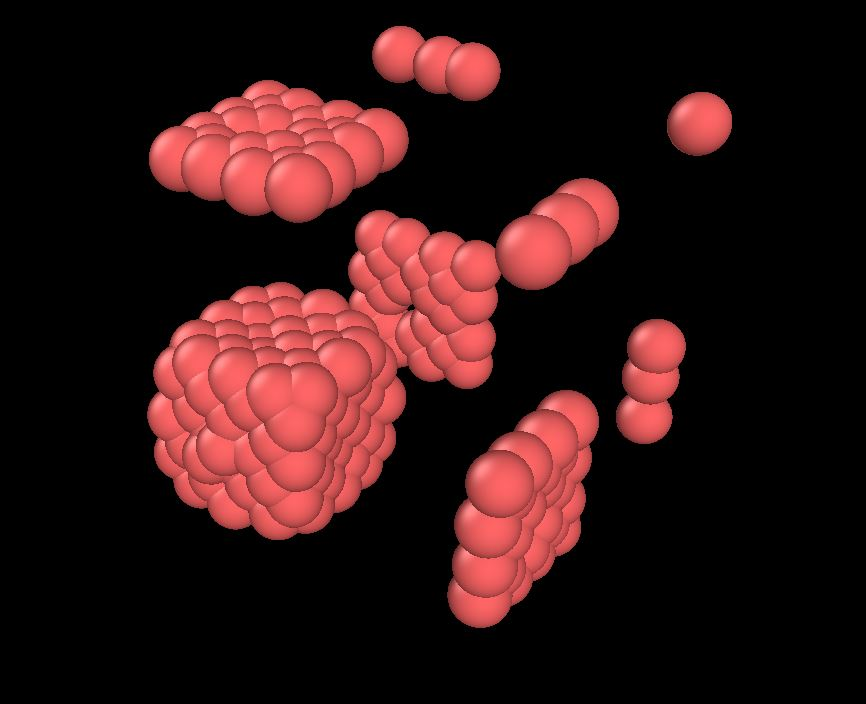
\includegraphics[scale=0.6]{./py/3di_3_ovito.jpg} 
        \caption{Periodic boundary conditions apparent}
        %Label gjør det enkelt å referere til ulike bilder.
        \label{fig:3di_2}
\end{figure}


\begin{figure}[h!]
        \centering 
        %Scale angir størrelsen på bildet. Bildefilen må ligge i samme mappe som tex-filen. 
        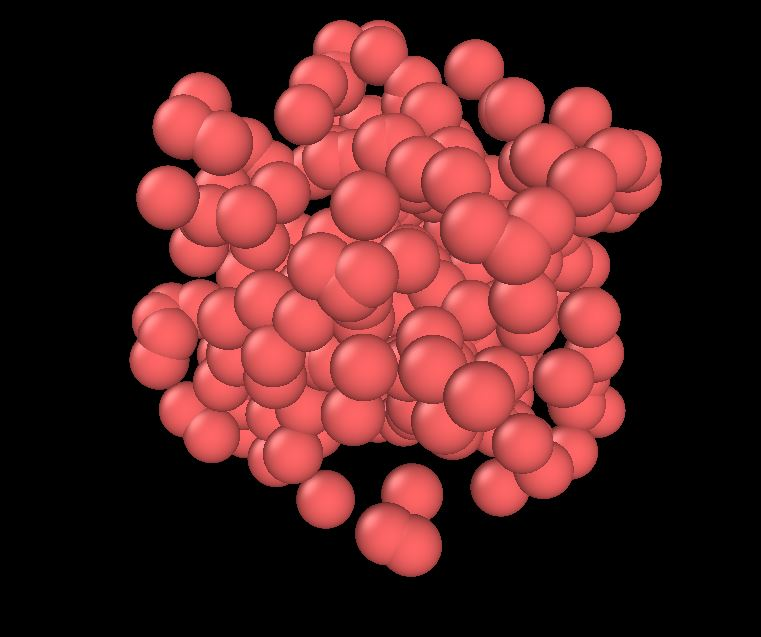
\includegraphics[scale=0.6]{./py/3di_2_ovito.jpg} 
        \caption{Crystal has expanded to fill box}
        %Label gjør det enkelt å referere til ulike bilder.
        \label{fig:3di_2}
\end{figure}


